
% Default to the notebook output style

    


% Inherit from the specified cell style.




    
\documentclass[11pt]{article}

    
    
    \usepackage[T1]{fontenc}
    % Nicer default font (+ math font) than Computer Modern for most use cases
    \usepackage{mathpazo}

    % Basic figure setup, for now with no caption control since it's done
    % automatically by Pandoc (which extracts ![](path) syntax from Markdown).
    \usepackage{graphicx}
    % We will generate all images so they have a width \maxwidth. This means
    % that they will get their normal width if they fit onto the page, but
    % are scaled down if they would overflow the margins.
    \makeatletter
    \def\maxwidth{\ifdim\Gin@nat@width>\linewidth\linewidth
    \else\Gin@nat@width\fi}
    \makeatother
    \let\Oldincludegraphics\includegraphics
    % Set max figure width to be 80% of text width, for now hardcoded.
    \renewcommand{\includegraphics}[1]{\Oldincludegraphics[width=.8\maxwidth]{#1}}
    % Ensure that by default, figures have no caption (until we provide a
    % proper Figure object with a Caption API and a way to capture that
    % in the conversion process - todo).
    \usepackage{caption}
    \DeclareCaptionLabelFormat{nolabel}{}
    \captionsetup{labelformat=nolabel}

    \usepackage{adjustbox} % Used to constrain images to a maximum size 
    \usepackage{xcolor} % Allow colors to be defined
    \usepackage{enumerate} % Needed for markdown enumerations to work
    \usepackage{geometry} % Used to adjust the document margins
    \usepackage{amsmath} % Equations
    \usepackage{amssymb} % Equations
    \usepackage{textcomp} % defines textquotesingle
    % Hack from http://tex.stackexchange.com/a/47451/13684:
    \AtBeginDocument{%
        \def\PYZsq{\textquotesingle}% Upright quotes in Pygmentized code
    }
    \usepackage{upquote} % Upright quotes for verbatim code
    \usepackage{eurosym} % defines \euro
    \usepackage[mathletters]{ucs} % Extended unicode (utf-8) support
    \usepackage[utf8x]{inputenc} % Allow utf-8 characters in the tex document
    \usepackage{fancyvrb} % verbatim replacement that allows latex
    \usepackage{grffile} % extends the file name processing of package graphics 
                         % to support a larger range 
    % The hyperref package gives us a pdf with properly built
    % internal navigation ('pdf bookmarks' for the table of contents,
    % internal cross-reference links, web links for URLs, etc.)
    \usepackage{hyperref}
    \usepackage{longtable} % longtable support required by pandoc >1.10
    \usepackage{booktabs}  % table support for pandoc > 1.12.2
    \usepackage[inline]{enumitem} % IRkernel/repr support (it uses the enumerate* environment)
    \usepackage[normalem]{ulem} % ulem is needed to support strikethroughs (\sout)
                                % normalem makes italics be italics, not underlines
    

    
    
    % Colors for the hyperref package
    \definecolor{urlcolor}{rgb}{0,.145,.698}
    \definecolor{linkcolor}{rgb}{.71,0.21,0.01}
    \definecolor{citecolor}{rgb}{.12,.54,.11}

    % ANSI colors
    \definecolor{ansi-black}{HTML}{3E424D}
    \definecolor{ansi-black-intense}{HTML}{282C36}
    \definecolor{ansi-red}{HTML}{E75C58}
    \definecolor{ansi-red-intense}{HTML}{B22B31}
    \definecolor{ansi-green}{HTML}{00A250}
    \definecolor{ansi-green-intense}{HTML}{007427}
    \definecolor{ansi-yellow}{HTML}{DDB62B}
    \definecolor{ansi-yellow-intense}{HTML}{B27D12}
    \definecolor{ansi-blue}{HTML}{208FFB}
    \definecolor{ansi-blue-intense}{HTML}{0065CA}
    \definecolor{ansi-magenta}{HTML}{D160C4}
    \definecolor{ansi-magenta-intense}{HTML}{A03196}
    \definecolor{ansi-cyan}{HTML}{60C6C8}
    \definecolor{ansi-cyan-intense}{HTML}{258F8F}
    \definecolor{ansi-white}{HTML}{C5C1B4}
    \definecolor{ansi-white-intense}{HTML}{A1A6B2}

    % commands and environments needed by pandoc snippets
    % extracted from the output of `pandoc -s`
    \providecommand{\tightlist}{%
      \setlength{\itemsep}{0pt}\setlength{\parskip}{0pt}}
    \DefineVerbatimEnvironment{Highlighting}{Verbatim}{commandchars=\\\{\}}
    % Add ',fontsize=\small' for more characters per line
    \newenvironment{Shaded}{}{}
    \newcommand{\KeywordTok}[1]{\textcolor[rgb]{0.00,0.44,0.13}{\textbf{{#1}}}}
    \newcommand{\DataTypeTok}[1]{\textcolor[rgb]{0.56,0.13,0.00}{{#1}}}
    \newcommand{\DecValTok}[1]{\textcolor[rgb]{0.25,0.63,0.44}{{#1}}}
    \newcommand{\BaseNTok}[1]{\textcolor[rgb]{0.25,0.63,0.44}{{#1}}}
    \newcommand{\FloatTok}[1]{\textcolor[rgb]{0.25,0.63,0.44}{{#1}}}
    \newcommand{\CharTok}[1]{\textcolor[rgb]{0.25,0.44,0.63}{{#1}}}
    \newcommand{\StringTok}[1]{\textcolor[rgb]{0.25,0.44,0.63}{{#1}}}
    \newcommand{\CommentTok}[1]{\textcolor[rgb]{0.38,0.63,0.69}{\textit{{#1}}}}
    \newcommand{\OtherTok}[1]{\textcolor[rgb]{0.00,0.44,0.13}{{#1}}}
    \newcommand{\AlertTok}[1]{\textcolor[rgb]{1.00,0.00,0.00}{\textbf{{#1}}}}
    \newcommand{\FunctionTok}[1]{\textcolor[rgb]{0.02,0.16,0.49}{{#1}}}
    \newcommand{\RegionMarkerTok}[1]{{#1}}
    \newcommand{\ErrorTok}[1]{\textcolor[rgb]{1.00,0.00,0.00}{\textbf{{#1}}}}
    \newcommand{\NormalTok}[1]{{#1}}
    
    % Additional commands for more recent versions of Pandoc
    \newcommand{\ConstantTok}[1]{\textcolor[rgb]{0.53,0.00,0.00}{{#1}}}
    \newcommand{\SpecialCharTok}[1]{\textcolor[rgb]{0.25,0.44,0.63}{{#1}}}
    \newcommand{\VerbatimStringTok}[1]{\textcolor[rgb]{0.25,0.44,0.63}{{#1}}}
    \newcommand{\SpecialStringTok}[1]{\textcolor[rgb]{0.73,0.40,0.53}{{#1}}}
    \newcommand{\ImportTok}[1]{{#1}}
    \newcommand{\DocumentationTok}[1]{\textcolor[rgb]{0.73,0.13,0.13}{\textit{{#1}}}}
    \newcommand{\AnnotationTok}[1]{\textcolor[rgb]{0.38,0.63,0.69}{\textbf{\textit{{#1}}}}}
    \newcommand{\CommentVarTok}[1]{\textcolor[rgb]{0.38,0.63,0.69}{\textbf{\textit{{#1}}}}}
    \newcommand{\VariableTok}[1]{\textcolor[rgb]{0.10,0.09,0.49}{{#1}}}
    \newcommand{\ControlFlowTok}[1]{\textcolor[rgb]{0.00,0.44,0.13}{\textbf{{#1}}}}
    \newcommand{\OperatorTok}[1]{\textcolor[rgb]{0.40,0.40,0.40}{{#1}}}
    \newcommand{\BuiltInTok}[1]{{#1}}
    \newcommand{\ExtensionTok}[1]{{#1}}
    \newcommand{\PreprocessorTok}[1]{\textcolor[rgb]{0.74,0.48,0.00}{{#1}}}
    \newcommand{\AttributeTok}[1]{\textcolor[rgb]{0.49,0.56,0.16}{{#1}}}
    \newcommand{\InformationTok}[1]{\textcolor[rgb]{0.38,0.63,0.69}{\textbf{\textit{{#1}}}}}
    \newcommand{\WarningTok}[1]{\textcolor[rgb]{0.38,0.63,0.69}{\textbf{\textit{{#1}}}}}
    
    
    % Define a nice break command that doesn't care if a line doesn't already
    % exist.
    \def\br{\hspace*{\fill} \\* }
    % Math Jax compatability definitions
    \def\gt{>}
    \def\lt{<}
    % Document parameters
    \title{main.py}
    
    
    

    % Pygments definitions
    
\makeatletter
\def\PY@reset{\let\PY@it=\relax \let\PY@bf=\relax%
    \let\PY@ul=\relax \let\PY@tc=\relax%
    \let\PY@bc=\relax \let\PY@ff=\relax}
\def\PY@tok#1{\csname PY@tok@#1\endcsname}
\def\PY@toks#1+{\ifx\relax#1\empty\else%
    \PY@tok{#1}\expandafter\PY@toks\fi}
\def\PY@do#1{\PY@bc{\PY@tc{\PY@ul{%
    \PY@it{\PY@bf{\PY@ff{#1}}}}}}}
\def\PY#1#2{\PY@reset\PY@toks#1+\relax+\PY@do{#2}}

\expandafter\def\csname PY@tok@sr\endcsname{\def\PY@tc##1{\textcolor[rgb]{0.73,0.40,0.53}{##1}}}
\expandafter\def\csname PY@tok@cp\endcsname{\def\PY@tc##1{\textcolor[rgb]{0.74,0.48,0.00}{##1}}}
\expandafter\def\csname PY@tok@gu\endcsname{\let\PY@bf=\textbf\def\PY@tc##1{\textcolor[rgb]{0.50,0.00,0.50}{##1}}}
\expandafter\def\csname PY@tok@fm\endcsname{\def\PY@tc##1{\textcolor[rgb]{0.00,0.00,1.00}{##1}}}
\expandafter\def\csname PY@tok@sd\endcsname{\let\PY@it=\textit\def\PY@tc##1{\textcolor[rgb]{0.73,0.13,0.13}{##1}}}
\expandafter\def\csname PY@tok@mo\endcsname{\def\PY@tc##1{\textcolor[rgb]{0.40,0.40,0.40}{##1}}}
\expandafter\def\csname PY@tok@dl\endcsname{\def\PY@tc##1{\textcolor[rgb]{0.73,0.13,0.13}{##1}}}
\expandafter\def\csname PY@tok@ss\endcsname{\def\PY@tc##1{\textcolor[rgb]{0.10,0.09,0.49}{##1}}}
\expandafter\def\csname PY@tok@ge\endcsname{\let\PY@it=\textit}
\expandafter\def\csname PY@tok@na\endcsname{\def\PY@tc##1{\textcolor[rgb]{0.49,0.56,0.16}{##1}}}
\expandafter\def\csname PY@tok@c\endcsname{\let\PY@it=\textit\def\PY@tc##1{\textcolor[rgb]{0.25,0.50,0.50}{##1}}}
\expandafter\def\csname PY@tok@sa\endcsname{\def\PY@tc##1{\textcolor[rgb]{0.73,0.13,0.13}{##1}}}
\expandafter\def\csname PY@tok@w\endcsname{\def\PY@tc##1{\textcolor[rgb]{0.73,0.73,0.73}{##1}}}
\expandafter\def\csname PY@tok@kn\endcsname{\let\PY@bf=\textbf\def\PY@tc##1{\textcolor[rgb]{0.00,0.50,0.00}{##1}}}
\expandafter\def\csname PY@tok@bp\endcsname{\def\PY@tc##1{\textcolor[rgb]{0.00,0.50,0.00}{##1}}}
\expandafter\def\csname PY@tok@gh\endcsname{\let\PY@bf=\textbf\def\PY@tc##1{\textcolor[rgb]{0.00,0.00,0.50}{##1}}}
\expandafter\def\csname PY@tok@sh\endcsname{\def\PY@tc##1{\textcolor[rgb]{0.73,0.13,0.13}{##1}}}
\expandafter\def\csname PY@tok@se\endcsname{\let\PY@bf=\textbf\def\PY@tc##1{\textcolor[rgb]{0.73,0.40,0.13}{##1}}}
\expandafter\def\csname PY@tok@kp\endcsname{\def\PY@tc##1{\textcolor[rgb]{0.00,0.50,0.00}{##1}}}
\expandafter\def\csname PY@tok@gt\endcsname{\def\PY@tc##1{\textcolor[rgb]{0.00,0.27,0.87}{##1}}}
\expandafter\def\csname PY@tok@sc\endcsname{\def\PY@tc##1{\textcolor[rgb]{0.73,0.13,0.13}{##1}}}
\expandafter\def\csname PY@tok@sb\endcsname{\def\PY@tc##1{\textcolor[rgb]{0.73,0.13,0.13}{##1}}}
\expandafter\def\csname PY@tok@m\endcsname{\def\PY@tc##1{\textcolor[rgb]{0.40,0.40,0.40}{##1}}}
\expandafter\def\csname PY@tok@gi\endcsname{\def\PY@tc##1{\textcolor[rgb]{0.00,0.63,0.00}{##1}}}
\expandafter\def\csname PY@tok@mi\endcsname{\def\PY@tc##1{\textcolor[rgb]{0.40,0.40,0.40}{##1}}}
\expandafter\def\csname PY@tok@nt\endcsname{\let\PY@bf=\textbf\def\PY@tc##1{\textcolor[rgb]{0.00,0.50,0.00}{##1}}}
\expandafter\def\csname PY@tok@il\endcsname{\def\PY@tc##1{\textcolor[rgb]{0.40,0.40,0.40}{##1}}}
\expandafter\def\csname PY@tok@ne\endcsname{\let\PY@bf=\textbf\def\PY@tc##1{\textcolor[rgb]{0.82,0.25,0.23}{##1}}}
\expandafter\def\csname PY@tok@gp\endcsname{\let\PY@bf=\textbf\def\PY@tc##1{\textcolor[rgb]{0.00,0.00,0.50}{##1}}}
\expandafter\def\csname PY@tok@kr\endcsname{\let\PY@bf=\textbf\def\PY@tc##1{\textcolor[rgb]{0.00,0.50,0.00}{##1}}}
\expandafter\def\csname PY@tok@si\endcsname{\let\PY@bf=\textbf\def\PY@tc##1{\textcolor[rgb]{0.73,0.40,0.53}{##1}}}
\expandafter\def\csname PY@tok@err\endcsname{\def\PY@bc##1{\setlength{\fboxsep}{0pt}\fcolorbox[rgb]{1.00,0.00,0.00}{1,1,1}{\strut ##1}}}
\expandafter\def\csname PY@tok@cm\endcsname{\let\PY@it=\textit\def\PY@tc##1{\textcolor[rgb]{0.25,0.50,0.50}{##1}}}
\expandafter\def\csname PY@tok@nl\endcsname{\def\PY@tc##1{\textcolor[rgb]{0.63,0.63,0.00}{##1}}}
\expandafter\def\csname PY@tok@nc\endcsname{\let\PY@bf=\textbf\def\PY@tc##1{\textcolor[rgb]{0.00,0.00,1.00}{##1}}}
\expandafter\def\csname PY@tok@vi\endcsname{\def\PY@tc##1{\textcolor[rgb]{0.10,0.09,0.49}{##1}}}
\expandafter\def\csname PY@tok@no\endcsname{\def\PY@tc##1{\textcolor[rgb]{0.53,0.00,0.00}{##1}}}
\expandafter\def\csname PY@tok@mh\endcsname{\def\PY@tc##1{\textcolor[rgb]{0.40,0.40,0.40}{##1}}}
\expandafter\def\csname PY@tok@vc\endcsname{\def\PY@tc##1{\textcolor[rgb]{0.10,0.09,0.49}{##1}}}
\expandafter\def\csname PY@tok@kc\endcsname{\let\PY@bf=\textbf\def\PY@tc##1{\textcolor[rgb]{0.00,0.50,0.00}{##1}}}
\expandafter\def\csname PY@tok@ow\endcsname{\let\PY@bf=\textbf\def\PY@tc##1{\textcolor[rgb]{0.67,0.13,1.00}{##1}}}
\expandafter\def\csname PY@tok@k\endcsname{\let\PY@bf=\textbf\def\PY@tc##1{\textcolor[rgb]{0.00,0.50,0.00}{##1}}}
\expandafter\def\csname PY@tok@cs\endcsname{\let\PY@it=\textit\def\PY@tc##1{\textcolor[rgb]{0.25,0.50,0.50}{##1}}}
\expandafter\def\csname PY@tok@nf\endcsname{\def\PY@tc##1{\textcolor[rgb]{0.00,0.00,1.00}{##1}}}
\expandafter\def\csname PY@tok@gs\endcsname{\let\PY@bf=\textbf}
\expandafter\def\csname PY@tok@nb\endcsname{\def\PY@tc##1{\textcolor[rgb]{0.00,0.50,0.00}{##1}}}
\expandafter\def\csname PY@tok@mb\endcsname{\def\PY@tc##1{\textcolor[rgb]{0.40,0.40,0.40}{##1}}}
\expandafter\def\csname PY@tok@kt\endcsname{\def\PY@tc##1{\textcolor[rgb]{0.69,0.00,0.25}{##1}}}
\expandafter\def\csname PY@tok@ni\endcsname{\let\PY@bf=\textbf\def\PY@tc##1{\textcolor[rgb]{0.60,0.60,0.60}{##1}}}
\expandafter\def\csname PY@tok@s\endcsname{\def\PY@tc##1{\textcolor[rgb]{0.73,0.13,0.13}{##1}}}
\expandafter\def\csname PY@tok@vg\endcsname{\def\PY@tc##1{\textcolor[rgb]{0.10,0.09,0.49}{##1}}}
\expandafter\def\csname PY@tok@vm\endcsname{\def\PY@tc##1{\textcolor[rgb]{0.10,0.09,0.49}{##1}}}
\expandafter\def\csname PY@tok@kd\endcsname{\let\PY@bf=\textbf\def\PY@tc##1{\textcolor[rgb]{0.00,0.50,0.00}{##1}}}
\expandafter\def\csname PY@tok@cpf\endcsname{\let\PY@it=\textit\def\PY@tc##1{\textcolor[rgb]{0.25,0.50,0.50}{##1}}}
\expandafter\def\csname PY@tok@o\endcsname{\def\PY@tc##1{\textcolor[rgb]{0.40,0.40,0.40}{##1}}}
\expandafter\def\csname PY@tok@gr\endcsname{\def\PY@tc##1{\textcolor[rgb]{1.00,0.00,0.00}{##1}}}
\expandafter\def\csname PY@tok@sx\endcsname{\def\PY@tc##1{\textcolor[rgb]{0.00,0.50,0.00}{##1}}}
\expandafter\def\csname PY@tok@nn\endcsname{\let\PY@bf=\textbf\def\PY@tc##1{\textcolor[rgb]{0.00,0.00,1.00}{##1}}}
\expandafter\def\csname PY@tok@mf\endcsname{\def\PY@tc##1{\textcolor[rgb]{0.40,0.40,0.40}{##1}}}
\expandafter\def\csname PY@tok@ch\endcsname{\let\PY@it=\textit\def\PY@tc##1{\textcolor[rgb]{0.25,0.50,0.50}{##1}}}
\expandafter\def\csname PY@tok@s1\endcsname{\def\PY@tc##1{\textcolor[rgb]{0.73,0.13,0.13}{##1}}}
\expandafter\def\csname PY@tok@nd\endcsname{\def\PY@tc##1{\textcolor[rgb]{0.67,0.13,1.00}{##1}}}
\expandafter\def\csname PY@tok@s2\endcsname{\def\PY@tc##1{\textcolor[rgb]{0.73,0.13,0.13}{##1}}}
\expandafter\def\csname PY@tok@c1\endcsname{\let\PY@it=\textit\def\PY@tc##1{\textcolor[rgb]{0.25,0.50,0.50}{##1}}}
\expandafter\def\csname PY@tok@go\endcsname{\def\PY@tc##1{\textcolor[rgb]{0.53,0.53,0.53}{##1}}}
\expandafter\def\csname PY@tok@nv\endcsname{\def\PY@tc##1{\textcolor[rgb]{0.10,0.09,0.49}{##1}}}
\expandafter\def\csname PY@tok@gd\endcsname{\def\PY@tc##1{\textcolor[rgb]{0.63,0.00,0.00}{##1}}}

\def\PYZbs{\char`\\}
\def\PYZus{\char`\_}
\def\PYZob{\char`\{}
\def\PYZcb{\char`\}}
\def\PYZca{\char`\^}
\def\PYZam{\char`\&}
\def\PYZlt{\char`\<}
\def\PYZgt{\char`\>}
\def\PYZsh{\char`\#}
\def\PYZpc{\char`\%}
\def\PYZdl{\char`\$}
\def\PYZhy{\char`\-}
\def\PYZsq{\char`\'}
\def\PYZdq{\char`\"}
\def\PYZti{\char`\~}
% for compatibility with earlier versions
\def\PYZat{@}
\def\PYZlb{[}
\def\PYZrb{]}
\makeatother


    % Exact colors from NB
    \definecolor{incolor}{rgb}{0.0, 0.0, 0.5}
    \definecolor{outcolor}{rgb}{0.545, 0.0, 0.0}



    
    % Prevent overflowing lines due to hard-to-break entities
    \sloppy 
    % Setup hyperref package
    \hypersetup{
      breaklinks=true,  % so long urls are correctly broken across lines
      colorlinks=true,
      urlcolor=urlcolor,
      linkcolor=linkcolor,
      citecolor=citecolor,
      }
    % Slightly bigger margins than the latex defaults
    
    \geometry{verbose,tmargin=1in,bmargin=1in,lmargin=1in,rmargin=1in}
    
    

    \begin{document}
    
    
    \maketitle
    
    

    
    Computational Lexical Semantics

LIN5580-SEM1-A-1718

Angelo Basile and Jovana Urosevic

January 31, 2018

\begin{longtable}[]{@{}l@{}}
\toprule
\endhead
\begin{minipage}[t]{0.07\columnwidth}\raggedright
\#\#\# Instruction on how to use this notebook to replicate the
results:\strut
\end{minipage}\tabularnewline
\begin{minipage}[t]{0.07\columnwidth}\raggedright
1. download and install python 2 2. download and install
\href{https://docs.pipenv.org/}{pipenv} 3. install cython separately:
\texttt{pipenv\ install\ cython} 4. install the requirements from the
Pipfile 5. active the virtualenvironment: \texttt{pipenv\ shell} 6.
\texttt{cd\ dissect-master} 7. install dissect:
\texttt{pipenv\ run\ python2\ setup.py\ install} 8. deactive the virtual
environment:\texttt{exit} 9. run the notebook:
\texttt{pipenv\ run\ jupyter\ notebook}\strut
\end{minipage}\tabularnewline
\bottomrule
\end{longtable}

    \begin{Verbatim}[commandchars=\\\{\}]
{\color{incolor}In [{\color{incolor}1}]:} \PY{c+c1}{\PYZsh{} confirm that dissect is installed correctly:}
        \PY{c+c1}{\PYZsh{} this import should give no errors}
        \PY{k+kn}{from} \PY{n+nn}{composes}\PY{n+nn}{.}\PY{n+nn}{semantic\PYZus{}space}\PY{n+nn}{.}\PY{n+nn}{space} \PY{k}{import} \PY{n}{Space}
\end{Verbatim}


    \begin{center}\rule{0.5\linewidth}{\linethickness}\end{center}

    \hypertarget{describe-the-distributional-hypothesis-and-explain-how-it-can-be-used-to-find-semantically-similar-words-in-corpora.-3-points}{%
\paragraph{1) Describe the Distributional Hypothesis and explain how it
can be used to find semantically similar words in corpora. (3
points)}\label{describe-the-distributional-hypothesis-and-explain-how-it-can-be-used-to-find-semantically-similar-words-in-corpora.-3-points}}

Distributional hypothesis was introduced by Harris (1968) and refers to
the relation between the word meaning and the context it appears in
(that is, the distribution of other words that accompany it and/or their
syntactic relations) (Jurafsky and Martin, 2017). If we can understand
the word meaning from the context it is commonly used in, then the words
with similar meaning should be very likely to appear in similar contexts
(ibid.).\\
   In order to see how this works in practice, we can look at the
example below:

\begin{enumerate}
\def\labelenumi{(\arabic{enumi})}
\tightlist
\item
   \emph{The woolly \textbf{lemur}, the aye aye and the ring tail
  \textbf{lemur} can be found on the island of Madagascar.\\
      \textbf{Lemurs} are best known for their large, round reflective
  eyes and their wailing screams.\\
      The biggest threat to the \textbf{lemur} is deforestation.}
\end{enumerate}

If we did not know what the word \emph{lemur} was, just based on these
sentences we could find out that it is an animal that lives on
Madagascar, that has big, round eyes and loud screams, that it probably
lives in the trees, etc. Besides this, if we take a look at the
concordance view in the corpus (example 2), not only will we see other
contexts that explain the word \emph{lemur}, but also other similar
words such as monkey, primate, species, etc. that frequently appear with
it.

\begin{enumerate}
\def\labelenumi{(\arabic{enumi})}
\setcounter{enumi}{1}
\tightlist
\item
  \emph{   -xxnigeoo-langren-20101250the lemur \textbf{monkey} or
     \textbf{lemur}       is surely an unique \textbf{animal} that is
  native\\
       forests, and provides homes for red ruffed            
  \textbf{lemur}       , \textbf{gorillas, colobus monkeys}, and
  \textbf{jaguars}\\
        Concreting the area in front of the new             
  \textbf{lemur}       enclosure we could have enough done over\\
       so now at gymnastics my ten year old is a           
  \textbf{lemur}       leaping a \textbf{cheetah} chasing a
  \textbf{spider} spanning\\
       \textbf{elephants, tigers (cubs), zebras, snakes},         
  \textbf{lemurs}      \textbf{monkeys, birds, kangaroos, ostriches},\\
       Really feel distrusted and alienated The             
  \textbf{lemur}       \textbf{monkey} is called so simply because it
  is\\
       Live here including 90\% of the world's the          
  \textbf{lemur}       \textbf{monkeys} . Madagascar is made up of}
\end{enumerate}

The fact that we can frequently see other words naming types of animals
around the word \emph{lemur}, points to a kind of a relation these words
have with our word \emph{lemur}. And if we look the word \emph{gorilla}
up in the corpus (example 3), we will again get quite similar words
around it in the context when it is used to refer to an animal (and not
as an attribute for a person): \emph{monkey, chimpanzee, animal,
species,} with the description of where and how it lives, etc. So quite
similar to the previous example. And this is what distributional
hypothesis is about - we can understand the meaning of a word from the
context, and we can find other similar words by looking at other similar
contexts (since gorilla and lemur have similar meaning, they will appear
in similar contexts).

(3)\emph{  to Goodison and hearing those \textbf{animals} doing
     \textbf{gorilla}      impressions than anything else Ive ever
heard.\\
    Important all-year-round foods of the lowland       
\textbf{gorilla}      in Gabon include the large ground-living\\
    of the feeding behaviour of the lowland             \textbf{gorilla}
     and its interaction with other fruit-eating\\
    the near relatives of man, the \textbf{chimpanzee} and
    \textbf{gorilla}      . In the case of these \textbf{species},
rigidly\\
    evolutionary ties with thee \textbf{chimpanzee} and
       \textbf{gorilla}      , but also his rather less obvious
resemblance\\
    relative, the \textbf{chimpanzee}, and even more in the    
\textbf{gorilla}      . But man is, in general, sexually dimorphic in\\
    are quite unlike anything found in the              \textbf{gorilla}
     or \textbf{chimpanzee}. They are, however, closely}\\
    In fact, in computational semantics, we can build distributional
semantic models to calculate similarity between certain words by
comparing the contexts they appear in (Jurafsky and Martin, 2017). The
idea is that the more contexts two words share, the more similar they
are. In DSMs, contexts are represented as vectors of co-occurrence
counts denoting how often words co-occur with one another (ibid.). Their
similarity is then calculated by comparing these vectors: if two words
have similar context vectors, then they have similar meaning (Basili and
Pennacchiotti, 2010; Jurafsky and Martin, 2017). These are high
dimensional, sparse vectors (containing many zeros) because most of the
words will just not happen to appear in the context of other words. This
vector representation of a word meaning is called embedding, while the
models trying to use words represented in this way are called
\emph{vector space models, word space models}, or \emph{vector based
models} (Van der Plas, 2017; Jurafsky and Martin, 2017).\\
   In order to calculate the similarity between terms, we can consider
the following example.

\begin{longtable}[]{@{}lllll@{}}
\toprule
& get & see & use & hear\tabularnewline
\midrule
\endhead
lemur & 5 & 35 & 2 & 22\tabularnewline
gorilla & 9 & 65 & 3 & 36\tabularnewline
cat & 35 & 74 & 5 & 40\tabularnewline
chair & 81 & 35 & 104 & 0\tabularnewline
\bottomrule
\end{longtable}

Table 1. Term-context matrix.

In the table we see a hypothetical example of co-occurrence counts for
the target words (raws) and their context words (columns). In order to
calculate the similarity between the target words given that they appear
in the context of the words \emph{get} and \emph{see}, we present them
in a n-dimensional (Euclidean) space (Evert, et al., 2010). The position
of the words is determined by their co-occurrence counts with the words
\emph{see} and \emph{get}: \emph{lemur = (10, 76)}.\\
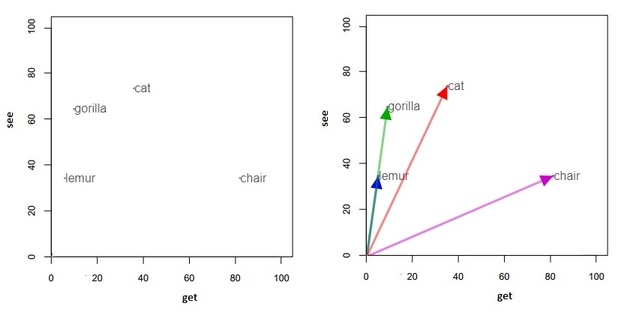
\includegraphics{pics/figure1.jpg}

Figure 1. Target words as points (left) or vectors (right) in
two-dimensional space.

There are several ways of counting similarity between the words now: by
either counting the Euclidean distance between the points (spatial
proximity), or by measuring the angle between the vectors (ibid.).
Measuring the angle is a better option because it takes into account
vector's direction rather than position of the word. For example, if we
take a look at the distance of the points in the figure 1 (left),
\emph{cat} and \emph{gorilla} will seem more similar than \emph{gorilla}
and \emph{lemur}. However, if we look at the angle between the vectors
on the right on the figure 1, we will notice that it is very small
between \emph{gorilla} and \emph{lemur}, showing their very close
similarity, as compared to the angle between \emph{gorilla} and
\emph{cat}, or in that matter \emph{chair}.

    \hypertarget{because-dsms-generate-ranked-lists-of-semantically-similar-words-they-can-be-seen-as-alternatives-to-manually-built-lexical-resources-such-as-wordnet.-5-points}{%
\paragraph{2) Because DSMs generate ranked lists of semantically similar
words, they can be seen as alternatives to manually built lexical
resources such as WordNet. (5
points)}\label{because-dsms-generate-ranked-lists-of-semantically-similar-words-they-can-be-seen-as-alternatives-to-manually-built-lexical-resources-such-as-wordnet.-5-points}}

\textbf{- Explain the main differences between the lexical semantic
content of WordNet and the lexical output of DSMs. }\\
WordNet is a type of a thesaurus in which not only can we find words'
definitions and their synonyms, but also other words they are related to
by a certain semantic relation (synonymy, hyponymy, polysemy, metonymy,
meronymy / holonymy, antonymy) (Miller et al, 1990). It contains open
class words (nouns, adjectives, verbs and adverbs) which are organized
by their senses and grouped into synonym sets (synsets). Besides, all
words are hierarchically structured in order to represent the semantic
relations between them (ibid.).\\
   Compared to the DSMs, when using WordNet it is relatively easy to
extract semantic relations between a target word and context words since
that information is explicitly represented in its structure. On the
other hand, when it comes to the output of a DSMs for a specific target
word, we get only a sorted list of most semantically related words
together with their scores, but without any information about what kind
of relation exists between the target word and the outputed words.\\
 \textbf{- Discuss advantages and drawbacks of manually built lexical
resources such as Wordnet and automatically generated lexical resources
such as lists of semantically similar words stemming from DSMs. }\\
When it comes to WordNet, one of its advantages is that it is hand-built
by linguist and therefore very precise (Van der Plas, 2017). However,
this kind of resource is expensive and time-consuming to create and can
also be quite difficult to maintain and keep updating for new words.
These are the reasons why it is difficult to have a similar resource for
other languages (ibid). Furthermore, it is definitely an advantage to
have explicit relations marked between different senses of words
together with glosses explaining the senses. One of the improvements
here could be to provide currently missing frequency information for the
synsets. If we take a look at WordNet, we will see that a lot of senses
following the first ones are quite infrequent in English language, but
no explicit information is given about this (ibid.). Also, when it comes
to relations between the synsets, most of them are represented as
binary, which is not the case for synonyms for example; there is a
higher or lower level of similarity / relatedness that is not quantified
in WordNet (ibid.). Here, words are either synonyms or not. This,
however, can be overcome using a thesaurus-based algorithms to calculate
words similarity given the hierarchical structure of WordNet, in which
case the similarity is calculated based on the distance of two words in
the hierarchy (Jurafsky and Martin, 2017).\\
   On the other hand, DSMs have their pros and cons as well. These
models are fast and inexpensive to obtain as opposed to WordNet
creation, and therefore can be applied to any domain and any language
(Van der Plas, 2017). Also, they provides a way to quantify semantic
relatedness between words (ibid.). However, the significant disadvantage
DSMs have compared to WordNet is that besides the similarity scores we
get in the output, we have no further information about the relations
between observed words. We do not get only synonyms in the outputs, but
all other sorts of semantic relations. Similarity in this approach is
taken quite broad and has as its disadvantage not being able to
distinguish between different relations, such as synonyms, antonyms,
etc. (Sahlgren, 2001).\\
 \textbf{- Can you think of an application that would fare better when
using WordNet and another that would benefit more from the output of
DSMs?}\\
WordNet is commonly used for the task of word sense disambiguation,
where we need to find the most appropriate sense of a word given the
context it appears in (Morato et al., 2004).\\
   DSMs could be used in many applications, such as in information
retrieval, where we can retrieve documents containing similar words to
the ones in a query. Also, it could be used in machine translation,
where DSMs could help us to find out if two words are similar enough to
be used in the same context, etc. (Jurafsky and Martin, 2017). inference
wn, johny snoring Johny sleeping, if one entails enothe, predict
entailment, snoring hyponym of sleeping, while

    \begin{longtable}[]{@{}l@{}}
\toprule
\endhead
\begin{minipage}[t]{0.09\columnwidth}\raggedright
\#\#\#\# In this assignment, in order to gather semantically similar
words, we will use the following: \textbf{1. Data:} - A monolingual
corpus: \textbf{English} - Word-aligned parallel texts for a language
pair \textbf{English-Spanish}\strut
\end{minipage}\tabularnewline
\begin{minipage}[t]{0.09\columnwidth}\raggedright
\textbf{2. Tools:} - an extraction program (for the extraction from the
parallel text): a program that gathers coocurrence counts for the target
words - a DSM tool, a program that will compute the similarity between
the coocurrence vectors for the head words we are interested in --
taking the coocurrence matrix as input\strut
\end{minipage}\tabularnewline
\bottomrule
\end{longtable}

    \hypertarget{building-a-coocurrence-matrix-from-a-corpus}{%
\paragraph{Building a coocurrence matrix from a
corpus:}\label{building-a-coocurrence-matrix-from-a-corpus}}

There are several ways to build a coocurrence matrix depending on the
target words you are selecting (parameter 1) and the type of features,
more in particular, the type of context you are selecting (parameter 2).
Please refer back to the slides of the lecture on DSMs for a list of
parameters and a description of the options.

\hypertarget{target-words}{%
\paragraph{\texorpdfstring{\emph{TARGET
WORDS}:}{TARGET WORDS:}}\label{target-words}}

    \hypertarget{does-the-monolingual-corpus-you-are-using-to-extract-the-cooccurrence-counts-from-provide-lemmas-discuss-why-using-lemmas-instead-of-words-often-leads-to-better-performances-in-dsms.-3-points}{%
\paragraph{3) Does the monolingual corpus you are using to extract the
cooccurrence counts from provide lemmas? Discuss why using lemmas
instead of words often leads to better performances in DSMs. (3
points)}\label{does-the-monolingual-corpus-you-are-using-to-extract-the-cooccurrence-counts-from-provide-lemmas-discuss-why-using-lemmas-instead-of-words-often-leads-to-better-performances-in-dsms.-3-points}}

The monolingual corpus we are using does not provide lemmas. However,
the lemmatization should be applied since it is a type of text
normalization that will help us reduce dimensionality, that is, avoid
data sparseness (Turney and Pantel, 2010). Here we are interested in
word similarity, and therefore we will want to convert all the different
grammatical forms of a certain word into one (lemma), since they all
carry essentially the same meaning. In this way, we will avoid counting
separately in the co-occurrence matrix different forms of the same word.
Lemmatization normally leads to a better performance because in this way
we are eliminating redundant grammatical information, while making it
easier to recognize semantic similarities among words (ibid.).

    \begin{center}\rule{0.5\linewidth}{\linethickness}\end{center}

\hypertarget{extra-points-the-parallel-text-does-not-provide-lemma-information-nor-pos-tags.-run-a-pos-tagger-on-both-sides-of-the-parallel-text-and-use-the-information-it-gives-you-for-the-dsm.-5-points}{%
\paragraph{4) Extra points: The parallel text does not provide lemma
information, nor PoS tags. Run a PoS tagger on (both sides of) the
parallel text and use the information it gives you for the DSM. (+5
points)}\label{extra-points-the-parallel-text-does-not-provide-lemma-information-nor-pos-tags.-run-a-pos-tagger-on-both-sides-of-the-parallel-text-and-use-the-information-it-gives-you-for-the-dsm.-5-points}}

    \textbf{The data provided with DISSECT already selected target words for
you. For the parallel text, and in case you selected your own
monolingual text, we take the 1550 most frequent content words (lemmas)
in the corpus as target words. In order to determine the 1550 most
frequent content words in either corpus, you will need to count all
content words. (If you do not have access to PoS information, use a list
of stopwords that you filter out.) You then need to rank these words
according to their frequency and take the top 1550.}

    \hypertarget{explain-why-pos-information-can-be-useful-for-distinguishing-between-ambiguous-terms.-give-some-examples-from-the-data-you-are-using.-3-points}{%
\paragraph{5) Explain why PoS information can be useful for
distinguishing between ambiguous terms. Give some examples from the data
you are using. (3
points)}\label{explain-why-pos-information-can-be-useful-for-distinguishing-between-ambiguous-terms.-give-some-examples-from-the-data-you-are-using.-3-points}}

POS information can be useful because it helps us disambiguate between
formally identical words with different meanings (Turney and Pantel,
2010). This does not refer to homonyms, but rather words that have the
same form only in certain contexts and are distinguishable by their
part-of-speech. For example, the word \emph{work} (noun,verb) without
POS information could be translated to Spanish as \emph{trabajo} (noun)
or \emph{trabajar} (verb). If we apply a POS-tagger on our data, we
avoid having this type of issue.\\
   Since we are working with a parallel corpus, not distinguishing
between different POS can mislead us into extracting wrong types of
translations into our co-occurrence matrix. The following examples are
from the Europarl English-Spanish parallel corpus that we are using. The
Spanish word \emph{poco} can have different translations into English
depending on its part-of-speech (example 4).

\begin{enumerate}
\def\labelenumi{(\arabic{enumi})}
\setcounter{enumi}{3}
\item
    \emph{(Spanish: determiner):   tienen dificultades con esta cuestión
  a dar esos \textbf{pocos} pasos más}\\
       \emph{(English: adjective):     who have difficulties in this
  matter to take those \textbf{few} extra steps}\\
       \emph{(Spanish: adverb):      Esto me molestó un \textbf{poco}
  porque}\\
       \emph{(English: adverb):      I was \textbf{somewhat} irritated
  about this} (informally could be also translated as \textbf{a bit, a
  little})\\
   In the opposite case, we can have English word \emph{well}
  differently translated depending on it POS information (example 5).
\item
  \emph{  (English: adverb):        this work has been carried out
  extremely \textbf{well}\\
       (Spanish: adverb):       Creo que es un trabajo muy \textbf{bien}
  realizado\\
       (English: interjection):    \textbf{Well}, we in Britain are
  looking to the European Court\\
       (Spanish: interjection):    \textbf{En fin} , en Gran Bretaña
  hemos recurrido\\
                              \textbf{Bien}, es verdad que se redactan
  regulaciones} (informally, it could also be also translated as
  \textbf{vaya, hala})\\
  \emph{     (English: noun):         is like carrying water to fill up
  a dry \textbf{well}\\
       (Spanish: noun)        es como si llevásemos agua al
  \textbf{pozo} }
\end{enumerate}

    \begin{center}\rule{0.5\linewidth}{\linethickness}\end{center}

\hypertarget{features}{%
\paragraph{\texorpdfstring{\emph{FEATURES}:}{FEATURES:}}\label{features}}

    \hypertarget{please-discuss-in-your-report-the-different-types-of-features-more-in-particular-the-types-of-context-parameter-2-that-are-employed-for-dsms-in-general.-5-points}{%
\paragraph{6) Please discuss in your report, the different types of
features, more in particular, the types of context (parameter 2) that
are employed for DSMs in general. (5
points)}\label{please-discuss-in-your-report-the-different-types-of-features-more-in-particular-the-types-of-context-parameter-2-that-are-employed-for-dsms-in-general.-5-points}}

As previously shown, DSMs are based on a co-occurrence matrix. There are
several types of co-occurrence matrices that we could build, such as
term-document matrix, term-context matrix and pair-pattern matrix
(Turney and Pantel, 2010; Jurafsky and Martin, 2017).\\
   \textbf{1. Term-document matrix.} In this kind of matrix rows
represent terms (words of the vocabulary), columns represent documents
(they can be actual documents of some kind or just a bigger collection
of text like web pages), while cells contain the number of times each
target word appears in each document (Jurafsky and Martin, 2017). In
this way, we have every document represented as a count vector or as a
point in a n-dimensional space. Two documents are considered to be
similar if they contain similar words, and therefore have similar
vectors (ibid.). As seen earlier, we can measure the similarity between
the documents either by measuring the distance between the points or by
measuring the angle between the vectors in the semantic space. The
smaller the angle or distance, the more similar two documents are. In
other words, the more similar words they contain, the more similar they
are.

\begin{longtable}[]{@{}llll@{}}
\toprule
& doc1 & doc2 & doc3\tabularnewline
\midrule
\endhead
lemur & 0 & 15 & 1\tabularnewline
gorilla & 0 & 21 & 2\tabularnewline
cat & 6 & 4 & 17\tabularnewline
chair & 12 & 0 & 0\tabularnewline
\bottomrule
\end{longtable}

Table 2. Term-document matrix.

    \textbf{2. Term-context matrix} (also called word-word or term-term
matrix).When it comes to term-context matrix, the rows of a matrix are
again target words (terms), while in the columns we have a narrower
context than previously used document, however it can refer to anything
from a whole vocabulary, certain words, paragraphs, sentences, to
specific syntactic relations among words (Evert et al., 2010; Van der
Plas, 2017). The following subsections summarize all \emph{context}
possibilities.\\
    ** - Surface context: **\\
This type of context refers to the ``window'' around the target word,
which basically consists of n words or characters to its left and n
words or characters to its right (ibid.). In this case, the cells in the
matrix contain counts of how many times the word in the column appeared
in the n-word window around the row (target) word. For example, if we
have the 7-word window around the words \emph{gorilla, lemur, cat} and
\emph{chair}, we get the following example sentences (obtained from the
British National Corpus):

(6)\emph{  with the consequent loss of habitat for       
\textbf{gorillas}   , elephants and other threatened animal\\
     that there is a home for owls and squirrels,    \textbf{lemurs}   ,
parrots and toucans. A river with slightly\\
     outback have been set back by domestic     \textbf{cats}      ,
which have killed 11 of the rare animals\\
     Kendal would you like to bring your          \textbf{chair}     
over. Rachael can you see the board from where}

Then, we can make a matrix (table 3) with the four target words in rows
and some exemplar context words in columns extracted from the 7-word
window (there are many more words that could be added to the matrix, but
this is just an example).

\begin{longtable}[]{@{}llllllll@{}}
\toprule
& \ldots{} & habitat & elephants & animal & squirrels & board &
\ldots{}\tabularnewline
\midrule
\endhead
lemurs & \ldots{} & 0 & 0 & 0 & 1 & 0 & \ldots{}\tabularnewline
gorillas & \ldots{} & 1 & 1 & 1 & 0 & 0 & \ldots{}\tabularnewline
cats & \ldots{} & 0 & 0 & 1 & 0 & 0 & \ldots{}\tabularnewline
chair & \ldots{} & 0 & 0 & 0 & 0 & 1 & \ldots{}\tabularnewline
\bottomrule
\end{longtable}

Table 3. Term-context matrix.

  The size of the window can be as small or as big as we need. Depending
on what kind of relations we want to extract, we will need one or the
other (Evert et al., 2010). More about how the window size can influence
the relations we can extract from corpus is in the question 7.
Furthermore, we can choose if we want to get both the left and the right
context, or only one of them, depending on if we are interested in the
words that follow or precede the target word, or both. For example, if
we wanted to see what kind of adjectives normally describe a lemma
\emph{woman}, then in that case we would want to extract only the left
context. And finally, we can chose to weight words that are closer or
further from the target word in the context, again depending on what
kind of information we want to extract; we can have either uniform or
distance-based weightening (Evert et al., 2010).\\
    ** - Textual context:**\\
This type of context refers to the fact that the context terms belong to
the same linguistic unit as the target term (Evert et al., 2010).
Commonly these linguistic units are sentences or paragraphs, but can
also be turns in a conversation or texts on web pages (Evert et al.,
2010; Van der Plas, 2017). This kind of context somewhat resolves the
problem surface context has: we need to choose a particular, fixed
number as a window size (Evert, 2008). This will not always fulfill our
expectations: window can sometimes be too big, and go over sentence or
paragraph boundaries, or too small and not catch the context we want.
For example, catching a context of \emph{throw} in a 3-word window will
catch \emph{throw a birthday party}, but not \emph{throw a big birthday
party} (Evert, 2008). This can be particularly problematic when working
with a language that has a more free word order and where closely
related words could appear far apart in the context. In those cases,
textual context would be more appropriate to use.\\
    \textbf{- Syntactic context:}\\
This type of context includes co-occurrence counts of the target words
and the words that have a specific syntactic relation with the target
words (Evert et al., 2010; Van der Plas, 2017). We can have different
types of relations such as subject, object, modifier, coordination,
apposition, etc. (ibid.). In this way, the columns of the matrix are
syntactic relations with specific words we are interested in, while the
cells contain how many times the target and the context word appeared in
a particular syntactic context (table 4). As compared to the surface
context, it does not set a strict word limit as context but it manages
to catch relations happening further away from the target word; while
compared to the textual context, it introduces less noise (Evert, 2008).

\begin{longtable}[]{@{}lllll@{}}
\toprule
& eat-subj & paint-obj & long-tailed-adj & have-obj\tabularnewline
\midrule
\endhead
lemur & 32 & 0 & 43 & 16\tabularnewline
gorilla & 35 & 0 & 9 & 17\tabularnewline
cat & 30 & 0 & 5 & 25\tabularnewline
chair & 0 & 20 & 0 & 24\tabularnewline
\bottomrule
\end{longtable}

Table 4. Term-context matrix: syntactic context.

    \textbf{- Multilingual or translational context}\\
When it comes to multilingual context, it contains as columns target
word translated to other languages, while cells contain how many times a
certain target word was translated in a particular way in a particular
language (Van der Plas, 2017). This kind of information we can extract
from aligned parallel corpora. For example:

\begin{longtable}[]{@{}lll@{}}
\toprule
& autunno-IT & herfst-NL\tabularnewline
\midrule
\endhead
fall & 8 & 13\tabularnewline
autumn & 10 & 8\tabularnewline
\bottomrule
\end{longtable}

Table 5. Term-context matrix: translational context.

Here we can see how many times the formal variations with the same
meaning \emph{autumn} and \emph{fall} were translated as such in Italian
and Dutch. Besides looking at different types of translations, in this
context we can also capture how a certain phrase or a word is expressed
in different languages.

   \textbf{3. Pair-pattern matrix.} The pair-pattern matrix is used to
measure similarity between different kind of patterns (Turney and
Pantel, 2010). In this matrix the columns represent the patterns, for
example \emph{X solves Y}, while the cells contain the counts of how
many times target words appear as a part of this pattern. As stated by
Lin and Pantel (2001) (in Turney and Pantel, 2010), pairs of target
words that co-occur with similar patterns, tend to have similar meaning.
The idea is that given the pattern X solves Y, we will find similar
patterns such as ``Y is solved by X'', ``Y is resolved in X'', and ``X
resolves Y'' (Turney and Pantel, 2010). That is, these patterns tend to
appear together with similar X and Y word pairs, which points to their
similar meaning. For example, pairs \emph{mason : stone, carpenter
:wood} appear with similar semantic relation \emph{artisan :material}
(Turney and Pantel, 2010).\\
    In summary, the more structured and restricted the context, the more
closely related are the words the system finds. Synonymy is a very tight
semantic relation, co-hyponymy and direct hyponymy a bit less, indirect
hyponymy even less. Mere association is the least semantically tight
relation. (Van der Plas, 2017)
\_\_\_\_\_\_\_\_\_\_\_\_\_\_\_\_\_\_\_\_\_\_\_\_\_\_\_\_\_\_\_

    \textbf{For the aligned parallel text, we are going to select the words
that are aligned to the target word as features. Please select only the
10000 most frequent content words as features. If you opted to include
your own monolingual corpus, we are going to select a small window of
the content word following and the content word preceding the target
word, as features. Please select only the 10000 most frequent content
words as features.}

    \hypertarget{discuss-what-influence-the-size-of-the-window-has-on-the-nature-of-the-semantic-relations-we-find-between-target-word-and-semantically-similar-words-proposed-by-the-system.-what-consequences-do-you-think-a-larger-window-size-would-have-on-the-semantically-similar-words-proposed-by-the-system-3-points}{%
\paragraph{7) Discuss what influence the size of the window has on the
nature of the semantic relations we find between target word and
semantically similar words proposed by the system. What consequences do
you think a larger window size would have on the semantically similar
words proposed by the system? (3
points)}\label{discuss-what-influence-the-size-of-the-window-has-on-the-nature-of-the-semantic-relations-we-find-between-target-word-and-semantically-similar-words-proposed-by-the-system.-what-consequences-do-you-think-a-larger-window-size-would-have-on-the-semantically-similar-words-proposed-by-the-system-3-points}}

Example from Evert et al. (2010), nearest neighbours for a word
\emph{dog} extracted from BNC with different window sizes:\\
(7)\\
    2-word window: \emph{cat, horse, fox, pet, rabbit, pig, animal,
mongrel, sheep, pigeon}\\
    30-word window: \emph{kennel, puppy, pet, bitch, terrier,
rottweiler, canine, cat, to bark, Alsatian}\\
 In general, the shorter the window, the more syntactic information we
catch since we are focusing only on the nearest neighbours of the target
word, while on the other hand, longer window catches more semantic
relations between the words (Jurafsky and Martin, 2017). In this sense,
we have two kinds of similarity as stated by Jurafsky and Martin (2017).
Firstly, we say that words have first-order co-occurrence (syntagmatic
association) when they are normally found near each other. For example,
that is the case with words \emph{book} and \emph{poem} with the verb
\emph{write}; they indeed normally appear close to one another and
\emph{book} and \emph{poem} are normally encountered as objects of the
verb \emph{write}. On the other hand, we have a second-order
co-occurrence (paradigmatic association) if the words have similar
neighbours (Jurafsky and Martin, 2017). For example, this is the case
with the word \emph{wrote} and words \emph{said}, \emph{told}, etc.\\
   When it comes to the type of a semantic relation depending on the
window size, when we have a shorter window, we catch similar words to
the target in the sense that it can appear in the similar syntactic
position. In the example given below, we get all sort of names for
animals when we look for the similar words for \emph{dog}: \emph{cat,
horse, pidgeon}, etc. With the wider window, we catch words like
\emph{dog} that are likely to appear in a similar text, in the text of a
similar topic: \emph{kennel, puppy, pet, bitch}. In the wider context,
we get synonyms for example, while in the narrower context we get
related words, hyponyms, hypernyms, ..\\
   The more restricted the context, the more closely related are the
words the system finds. The larger window allows us to capture a bit
further semantic relations. the wider the context the bigger chance is
for us to find synonyms since they will not normally occur one after
another

Presentation: The more structured and restricted the context, the more
closely related are the words the system finds. Synonymy is a very tight
semantic relation, co-hyponymy and direct hyponymy a bit less, indirect
hyponymy even less. Mere association is the least semantically tight
relation.:

    \hypertarget{discuss-the-differences-in-output-of-the-dsm-in-terms-of-the-similar-words-it-will-produce-you-expect-between-the-two-types-of-input-you-are-using-the-monolingual-corpus-and-the-aligned-parallel-files.-which-type-of-data-do-you-think-will-generate-the-highest-percentage-of-synonyms-amongst-the-nearest-neighbours-3-points}{%
\paragraph{8) Discuss the differences in output of the DSM (in terms of
the similar words it will produce) you expect between the two types of
input you are using (the monolingual corpus and the aligned parallel
files). Which type of data do you think will generate the highest
percentage of synonyms amongst the nearest neighbours? (3
points)}\label{discuss-the-differences-in-output-of-the-dsm-in-terms-of-the-similar-words-it-will-produce-you-expect-between-the-two-types-of-input-you-are-using-the-monolingual-corpus-and-the-aligned-parallel-files.-which-type-of-data-do-you-think-will-generate-the-highest-percentage-of-synonyms-amongst-the-nearest-neighbours-3-points}}

    \begin{center}\rule{0.5\linewidth}{\linethickness}\end{center}

\hypertarget{write-a-python-program-that-extracts-coocurrence-counts-for-all-target-words-and-features-from-the-parallel-aligned-files-and-the-monolingual-corpus-if-you-are-using-a-different-corpus-than-the-one-provided-by-dissect.-include-the-extraction-program-you-wrote-in-the-submission-and-paste-20-lines-for-20-target-words-of-the-coocurrence-counts-you-extracted-in-the-report.-the-output-of-your-program-should-be-formatted-according-to-the-input-format-the-dsm-tool-you-are-using-requires.-36-points}{%
\paragraph{9) Write a python program that extracts coocurrence counts
for all target words and features from the parallel aligned files (and
the monolingual corpus, if you are using a different corpus than the one
provided by DISSECT). Include the extraction program you wrote in the
submission, and paste 20 lines (for 20 target words) of the coocurrence
counts you extracted in the report. The output of your program should be
formatted according to the input format the DSM tool you are using
requires. (36
points)}\label{write-a-python-program-that-extracts-coocurrence-counts-for-all-target-words-and-features-from-the-parallel-aligned-files-and-the-monolingual-corpus-if-you-are-using-a-different-corpus-than-the-one-provided-by-dissect.-include-the-extraction-program-you-wrote-in-the-submission-and-paste-20-lines-for-20-target-words-of-the-coocurrence-counts-you-extracted-in-the-report.-the-output-of-your-program-should-be-formatted-according-to-the-input-format-the-dsm-tool-you-are-using-requires.-36-points}}

    \begin{center}\rule{0.5\linewidth}{\linethickness}\end{center}

\hypertarget{feature-weighting-and-similarity-function}{%
\paragraph{\texorpdfstring{\emph{Feature weighting and similarity
function:}}{Feature weighting and similarity function:}}\label{feature-weighting-and-similarity-function}}

    \hypertarget{explain-what-function-the-feature-weighting-scheme-has.-what-would-be-the-drawback-of-doing-without-a-weighting-scheme-and-using-raw-frequencies-instead-3-points}{%
\paragraph{10) Explain what function the feature weighting scheme has.
What would be the drawback of doing without a weighting scheme and using
raw frequencies instead? (3
points)}\label{explain-what-function-the-feature-weighting-scheme-has.-what-would-be-the-drawback-of-doing-without-a-weighting-scheme-and-using-raw-frequencies-instead-3-points}}

When working with language and having a big collection of words as
features, we commonly end up with having a very noisy feature
representation, which means that we have a lot of features that are
redundant and not very informative for the task we are trying to
conduct. The purpose of using a measure of feature weighting is to
reassign new counts to the co-occurrence matrix, but this time taking
into account how informative they are for our task. For example, if we
just take raw counts into consideration, it will turn out that frequent
words, such as \emph{the, a it, about, on, for}, etc. (stop words),
appear very frequently in a lot of contexts and therefore mislead us
into thinking that they are similar with a lot of different kind of
words just because they appear very frequently. So the raw counts are
not the best measure of similarity between words (Jurafsky and Martin,
2017; Van der Plas, 2017) and can many times mislead us. Also, for
example, if we are trying to figure out what kind of context is shared
between \emph{gorilla} and \emph{lemur} but not by \emph{chair} and
\emph{table} we will not get a lot of information from the stop words
mentioned earlier, that will appear in a lot of contexts and with many
different words and therefore cannot tell us anything in particular
about any target word. Since this is the case and we would like to
extract the most informative context words, we need to measure the
informativeness of words we want to use.\\
   There are several weightnening measures we can use, for example
Pointwise mutual information or log-likelihood ratio. These are
association measures of ``how much more often than chance two words
co-occur'' (Jurafsky and Martin, 2017), that is it weights the
association between the target word and the features by comparing the
expected and the observed co-occurrence frequency (Van der Plas, 2017).
``The less frequent the target word and the context feature are, the
higher the weight given to their observed co-occurrence count should be
(because their expected chance co-occurrence frequency is low)'' (Evert
et al., 2010).\\
   Another very known feature weighting method is tf-idf. It is not much
used when measuring semantic similarity, but it is used in many other
applications, especially information retrieval where it is a dominant
method for weighting frequencies. (Jurafsky and Martin, 2010). What it
does is that it give less weight to the features that appear in a lot of
different documents, because that means they are not very informative
for distinguishing between different types of documents. Fro the words
that appear not as often and in only certain type of document, more
weight is given since it shows that they are a good indicator of that
document type (ibid.). So more weight is given to a term frequent in a
certain document type, but rare in general in other documents.

    \hypertarget{list-the-weighting-schemes-the-tool-you-are-using-includes-and-what-similarity-functions.-make-your-choice-for-the-weighting-scheme-and-similarity-function-you-will-use-and-motivate-your-choice-in-the-report.-3-points}{%
\paragraph{11) List the weighting schemes the tool you are using
includes and what similarity functions. Make your choice for the
weighting scheme and similarity function you will use and motivate your
choice in the report. (3
points)}\label{list-the-weighting-schemes-the-tool-you-are-using-includes-and-what-similarity-functions.-make-your-choice-for-the-weighting-scheme-and-similarity-function-you-will-use-and-motivate-your-choice-in-the-report.-3-points}}

    \begin{center}\rule{0.5\linewidth}{\linethickness}\end{center}

\hypertarget{analysing-the-output}{%
\paragraph{\texorpdfstring{\emph{Analysing the
output:}}{Analysing the output:}}\label{analysing-the-output}}

    \textbf{Now we are ready to generate some output. You should be able to
get the distributional similar words of any of the 1550 target words you
selected.}

    \hypertarget{for-both-types-of-corpora-multilingual-and-monolingual-retrieve-the-top-5-semantically-similar-words-for-five-high-frequency-words-and-five-low-frequency-words-from-the-1550-words.-paste-the-output-in-the-report.}{%
\paragraph{12) For both types of corpora (multilingual and monolingual),
retrieve the top-5 semantically similar words for five high-frequency
words and five low-frequency words from the 1550 words. Paste the output
in the
report.}\label{for-both-types-of-corpora-multilingual-and-monolingual-retrieve-the-top-5-semantically-similar-words-for-five-high-frequency-words-and-five-low-frequency-words-from-the-1550-words.-paste-the-output-in-the-report.}}

\begin{itemize}
\tightlist
\item
  Is there a difference in the quality of the output for the
  high-frequency versus the low-frequency words?
\item
  Is there a difference for the two types of contexts used? Can you
  explain what you see? (5 points)
\end{itemize}

    \hypertarget{explain-the-notion-of-contextual-variability.}{%
\paragraph{13) Explain the notion of contextual
variability.}\label{explain-the-notion-of-contextual-variability.}}

Take a polysemous word of your choice that is among the 1550 head words
you selected. Generate the top-10 semantically similar words for this
target word using the monolingual DSM you created. Paste the output in
the report.\\
\textbf{- Do you see some consequences of contextual variability in the
outputs for this word?}\\
Now take the multilingual DSM. Find a polysemous word in the features of
the multilingual DSM1. For its translation in your target language, find
the top-10.\\
\textbf{- What are your observations?}\\
\textbf{- Do you think using multiple languages could have improved the
multilingual DSM? (5 points)}

    \begin{center}\rule{0.5\linewidth}{\linethickness}\end{center}

\hypertarget{compositionality}{%
\paragraph{\texorpdfstring{\emph{Compositionality:}}{Compositionality:}}\label{compositionality}}

    \hypertarget{explain-the-principle-of-compositionality-and-discuss-a-couple-of-different-ways-in-which-dsms-have-been-adapted-to-cater-for-compositionality.-3-points}{%
\paragraph{14) Explain the principle of compositionality and discuss a
couple of different ways in which DSMs have been adapted to cater for
compositionality. (3
points)}\label{explain-the-principle-of-compositionality-and-discuss-a-couple-of-different-ways-in-which-dsms-have-been-adapted-to-cater-for-compositionality.-3-points}}

Most of the work done in Distributional semantics takes into account
only single, isolated words (Guevara, 2011). However, in language we
combine words into bigger structures, phrases and sentences, such as
\emph{strong coffee, table cloth, hot dog}, etc. (Van der Plas, 2017).
Therefore, we would want DSMs to be able to deal with these more complex
structures as well. This is where the compositionality theory comes in
place, which is the fundamental idea in most of the contemporary works
in semantics (Van der Plas, 2017). It is based on the Principle of
compositionality: the meaning of a complex expression is comprised of
the meaning of its parts and by the syntactic rules that combine them
(Partee, ter Meulen and Wall, 1990: 318 in Guevara, 2011).\\
   So the question rises how to deal with compositionality in DSMs. This
is not an easy task and if we take a look at the compounds as a quite
good example of how problematic compositionality is, we will see that
there are several levels of compositionality (Van der Plas, 2017). Some
compounds can have somewhat compositional meaning, as in \emph{table
cloth}, others can have it partially compositional as \emph{data base},
while some will have a meaning that cannot be split into meaningful
parts as in \emph{hot dog}. Besides, they could consist of combinations
of different parts of speech ADJ-N, N-N, V-N, etc. (ibid.).\\
? Verbs + Prepositions: I e.g.~the difference between to stand on and to
stand up I Phrasal compositionality: I e.g.~red car\\
   Previous research has had several ideas to tackle the problem of
compositionality using DSMs models. Firstly, the attempt was made to
treat complex expressions as a whole unit, since some of them already
are merged together as for example database or compounds in general in
German language. Following the Distributional hypothesis, we could then
represent the meaning of a compound by looking at all the contexts it
appears in. However, the problem with this approach is that it works
only when looking into a really large corpus of text and with only very
frequent compounds, so data sparsity would be an issue since the rare
compounds would be quite bad representations (Van der Plas, 2017).
Besides, even with the frequent compounds there an issue of be able to
``generalize or reuse word meaning in a transparent use'' (ibid.).\\
   Given all the issues previously stated, the work done after this
treat compositionality as a function, which means that given to
independent vectors, the semantically compositional resulting vector is
created by one of the following operations: vector addition, (pointwise)
vector multiplication or tensor product (Guevara, 2011; Van der Plas,
2017). Vector addition is one of the most common approaches in the
literature introduced by Mitchell and Lapata (2010) (as stated in Van
der Plas, 2017)) and it involves a simple addition as follows:

\begin{enumerate}
\def\labelenumi{(\arabic{enumi})}
\setcounter{enumi}{2}
\tightlist
\item
  summation: v1 + v2 = v3\\
     red {[}1 2 0{]} + house {[}14 16 20{]} = red house {[}15 18 20{]}\\
      multiplication: v1 x v2 = v3\\
     red {[}1 2 0{]} x house {[}14 16 20{]} = red house {[}14 32 20{]}\\
      tensor product: v1⊗v2 = v3\\
     red = {[}1 2 0{]} ⊗ house = {[}0 1 3{]} = red house {[}1*0, 1*1,
  1*3, 2*0, 2*1, 2*3, 0*0, 0*1, 0*3{]} = red house {[}0, 1, 3, 0, 2, 6,
  0, 0, 0{]}\\
   So given two vectors v1 and v2, we get a compositional meaning of v3
  by summing the previous two up. Summing vectors is computationally
  efficient, however it does not provide us with an ideal solution (Van
  der Plas, 2017): the new vector is in between the two, but is more
  governed by the one that contains higher individual frequency counts.
  In the example of the \emph{red house}, the new vector is more
  influenced by the vector \emph{house} than the vector \emph{red}.
  Therefore, it resembles more a union than an intersection (ibid.).\\
     Mitchell and Lapata (2010) introduced also pointwise-multiplication
  of vectors. It differs from the addition model by only taking into
  account non-zero components of the vectors while the summation
  considers all of the components. The intuition is similar, we multiply
  two vectors and get as an output a third one that should correspond to
  the complex expression.\\
     Widdows (2008) (in Guevara, 2011) introduces a more complex vector
  operation, tensor product in order to capture meaning
  compositionality. The result of a tensor product of two vectors is a
  high dimensional matrix, which was shown empirically to catch better
  the compositionality of meaning (Van der Plas, 2017).\\
     All of the previously mentioned approaches have one thing in
  common: they all apply one single geometric operation on the vectors
  v1 and v2; it seems unlikely that only one operation can work on all
  semantic and syntactic relations and in all languages (Guevara, 2011).
\end{enumerate}

    \hypertarget{now-let-us-experiment-with-compositionality-in-the-monolingual-dsm-you-have-just-built.-follow-the-instructions-on-httpclic.cimec.unitn.itcomposestoolkitcomposing.html-and-select-a-model-of-your-choice-motivate-your-choice.-show-some-example-output-of-the-composed-dsm.-analyse-the-results.-5-points}{%
\paragraph{15) Now, let us experiment with compositionality in the
monolingual DSM you have just built. Follow the instructions on
http://clic.cimec.unitn.it/composes/toolkit/composing.html and select a
model of your choice (motivate your choice). Show some example output of
the composed DSM. Analyse the results. (5
points)}\label{now-let-us-experiment-with-compositionality-in-the-monolingual-dsm-you-have-just-built.-follow-the-instructions-on-httpclic.cimec.unitn.itcomposestoolkitcomposing.html-and-select-a-model-of-your-choice-motivate-your-choice.-show-some-example-output-of-the-composed-dsm.-analyse-the-results.-5-points}}

    \hypertarget{is-it-possible-to-create-a-compositional-model-for-the-multilingual-dsm-with-the-models-you-have-chosen-if-so-show-some-example-output-here-as-well.-analyse-the-results.-5-points}{%
\paragraph{16) Is it possible to create a compositional model for the
multilingual DSM with the models you have chosen? If so, show some
example output here as well. Analyse the results. (5
points)}\label{is-it-possible-to-create-a-compositional-model-for-the-multilingual-dsm-with-the-models-you-have-chosen-if-so-show-some-example-output-here-as-well.-analyse-the-results.-5-points}}

    \begin{center}\rule{0.5\linewidth}{\linethickness}\end{center}

\hypertarget{relating-things-back-to-theory}{%
\paragraph{\texorpdfstring{\emph{Relating things back to
theory:}}{Relating things back to theory:}}\label{relating-things-back-to-theory}}

    \textbf{We discussed several theories in class that try to explain the
lexical semantics of words. We are now trying to couple our knowledge
from one of these theories to the things we observe in the DSM. 1 For
example, if English is your target language and you chose German as the
counterpart in the parallel text, you could choose Kiefer in German (see
slides). One of its translations in English is pine. Now, get the top-10
most similar words of pine in the multilingual DSM and describe if you
see any unexpected nearest neighbours. You can try with several
polysemous words, if you like.}

    \hypertarget{discuss-the-basic-tenet-of-the-prototype-theory-in-lexical-semantics-and-discuss-at-least-two-advantages-when-compared-to-the-classical-theory.-5-points}{%
\paragraph{17) Discuss the basic tenet of the Prototype Theory in
lexical semantics and discuss at least two advantages when compared to
the classical theory. (5
points)}\label{discuss-the-basic-tenet-of-the-prototype-theory-in-lexical-semantics-and-discuss-at-least-two-advantages-when-compared-to-the-classical-theory.-5-points}}

The Prototype Theory emerged as a reaction to the problem with
psychological data in the Classical theory providing an alternative
approach (Laurence and Margolis, 1999). Even though there is not one
single prototype theory all theorists agree about, the general idea is
the same: ``most concepts - including most lexical concepts - are
complex representations whose structure encodes a statistical analysis
of the properties their members tend to have'' (ibid.). In other words,
most items in the extension of a concept will have these kind of
features ``typical'' of a concept, however there will be some items that
will not be represented by all of the ``typical'' features and yet still
belong to the same concept. This points to the fact that not all
features are by default necessary and that some of them are more
important than others (Van der Plas, 2017). This is different than what
the Classical theory suggests - that all features are necessary and that
an item has to satisfy all of concept's features in order to belong
under a certain concept (Laurence and Margolis, 1999). On the contrary,
the Prototype theory suggests satisfying a sufficient number of features
out of which some carry more importance than others (ibid.). For
example, if \emph{bird} is composed by features such as \emph{flies,
sings, has feathers, lays eggs, nests in trees}, etc. then we could say
that a \emph{sparrow} is a bird because it has all of the features. The
problem in the Classical theory would come up with birds such as
\emph{ostrich} since it does not have all the features therefore would
not be considered a bird. The Prototype theory takes care of these kind
of examples because even though \emph{ostrich} does not have all the
features, it has enough to be considered a bird - they do not fly, but
they have feathers, lay eggs, etc. An item that satisfies all the
features, or most of them, could be considered a prototypical example of
a concept.\\
   The previously stated rejection of the idea about ``necessary and
sufficient conditions'' goes along with Wittgenstein's idea that things
that fall under the same concept form ``a complicated network of
similarities overlapping and crisscrossing: sometimes overall
similarities, sometimes similarities of detail'' (Laurence and Margolis,
1999), in other words they have a ``family resemblance''. Rosch and
Mervis (1975, as stated in Laurence and Margolis, 1999) explain this
further: ``formal criteria are neither a logical nor psychological
necessity; the categorical relationship in categories which do not
appear to possess criterial attributes {[}\ldots{}{]} can be understood
in terms of the principle of family resemblance.'' In other words, they
all state that concepts are not governed by definitions but by a unfixed
set of properties that will appear in different combinations with
different items under a certain concept. The example they give is
\emph{game}; some games will one set of properties, some will have
other, but no matter what exact set of properties they have, what makes
them similar and to fall under the same concept is that their properties
overlap in a way that creates a similarity space (Laurence and Margolis,
1999). So what makes a certain game fall under the concept \emph{game}
is that it is within boundaries of this similarity space (ibid.).\\
   Since the Prototype theory was created mostly as a response to the
classical theory, it solves some of its problems one of which was
mentioned before about family resemblance and no need for a definition
of concepts. This lack of definitions is the problem the Classical
theory had that the Prototype theory successfully tackled by claiming
and proving that concepts do not have a definitional structure (Laurence
and Margolis, 1999). Second advantage the Prototype theory has over the
Classical theory is ts treatment of categorization, which tackles the
issues the latter theory had: conceptual fuzziness and typicality effect
(ibid.). Conceptual fuzziness refers to the problem of many concepts
being inexact (as \emph{carpet} belonging or not to the concept of
\emph{furniture}), while the typicality effects refer to the problems
where we have items that are not typical examples of a concept and
therefore do not have all the features it could have under a certain
concept (moer typical fruit: \emph{apple} or \emph{olive}) (Van der
Plas, 2017). The Prototype theory puts into a certain category an
instance if the representation of that instance is sufficiently similar
to the representation of the category (Laurence and Margolis, 1999). In
other words, it compares an instance with a prototypical example of the
category and if there is enough feature overlap, then they are similar
and belong to the same category. They have developed different types of
measures of similarity: they compare all the features in parallel and
depending on feature, it can add either a positive or a negative value
to the ``calculation'' depending if it is a common feature or not. If
the result obtained is not high enough to make a decision about whether
an instance belongs or not to a certain category, they just do not make
a judgement. And in their idea, this solves the fuzziness problem, they
just do not make any positive or negative judgment if there is not
enough evidence and are ok with the fact that some instances can be
somewhere in between (Laurence and Margolis, 1999).

    \hypertarget{what-are-typicality-effects-does-the-dsm-cater-for-typicality-effects-5-points}{%
\paragraph{18) What are typicality effects? Does the DSM cater for
typicality effects? (5
points)}\label{what-are-typicality-effects-does-the-dsm-cater-for-typicality-effects-5-points}}

The typicality effect refers to the fact that not all the members of a
certain category are equally typical examples of that category (Laurence
and Margolis, 1999; Connell and Ramscar, 2001). As stated in Laurence
and Margolis (1999), this was first proven by Rosch (1973) who found
that the participants in the study were able to rank items as more or
less typical members of a certain category. The example given to the
participants was to sort different types of fruits (\emph{apple, fig,
plum, olive}) on the 7-point scale by how well they represent the
category \emph{fruit}, which showed that certain fruits are commonly
addressed as typical (\emph{apple}), while others were marked as
atypical (\emph{olive}) (ibid.).\\
   If we take a look at the distributional similarity of these fruits,
we get the following output:

\begin{longtable}[]{@{}llll@{}}
\toprule
apple & plum & olive & fruit\tabularnewline
\midrule
\endhead
strawberry 0.808 & cherry 0.806 & olive 0.819 & berry
0.83\tabularnewline
pear 0.793 & pear 0.770 & almond 0.69 & mango 0.71\tabularnewline
cherry 0.780 & apricot 0.769 & olive 0.663 & vegetable
0.71\tabularnewline
peach 0.760 & apple 0.746 & carob 0.652 & drupe 0.70\tabularnewline
plum 0.746 & strawberry 0.739 & apricot 0.650 & flower
0.69\tabularnewline
apricot 0.744 & peach 0.736 & pistachio 0.631 & apple
0.69\tabularnewline
almond 0.740 & quince 0.735 & citrus 0.628 & strawberry
0.68\tabularnewline
quince 0.707 & persimmon 0.734 & avocado 0.627 & pear
0.68\tabularnewline
watermelon 0.705 & raspberry 0.705 & cinnamon 0.623 & apricot
0.68\tabularnewline
mango 0.694 & blackberry 0.699 & pomegranate 0.616 & pome
0.68\tabularnewline
\bottomrule
\end{longtable}

10 nearest neighbours Checked here
http://vectors.nlpl.eu/explore/embeddings/en/\# (computed from Wikipedia
(en))

   We will see that for the more typical fruits chosen by participants
(\emph{apple, plum}) we get similar distributional results, while for
the \emph{olive} (atypical example), we get a completely different set
of nouns (that we could argue share more properties with the olive
``oily''). And also, we see that \emph{apple} does appear as one of the
typical neighbours of \emph{fruit} while \emph{olive} does not. Since
the distributional similarity depends on the context these words appear
in, we could say that the more typical examples of fruits tend to appear
in different types of context than the non-typical ones.

    \begin{center}\rule{0.5\linewidth}{\linethickness}\end{center}

\hypertarget{team-work-distribution-by-assignment-questions}{%
\subsubsection{Team work distribution by assignment
questions:}\label{team-work-distribution-by-assignment-questions}}

\begin{itemize}
\item
  \textbf{Angelo}:\\
  1, 4, 5, 7, 11, 13, 14
\item
  \textbf{Jovana}:\\
  2, 3, 6, 8, 10, 12, 17
\item
  \textbf{Together:}\\
  9, 18, compositionality / embeddings
\end{itemize}

    \begin{center}\rule{0.5\linewidth}{\linethickness}\end{center}

\hypertarget{references}{%
\subsubsection{References}\label{references}}

\begin{itemize}
\tightlist
\item
  Basili, Roberto and Marco Pennacchiotti. (2010). Distributional
  lexical semantics: Toward uniform representation paradigms for
  advanced acquisition and processing tasks. In: Natural Language
  Engineering, 16 (4), pp.~347--358, 2010.\\
\item
  Connell, Louise and Michael Ramscar. (2001). Using Distributional
  Measures to Model Typicality in Categorization. \emph{In Proceedings
  of the 23rd Annual Conference of the Cognitive Science Society}.
  University of Edinburgh.\\
\item
  Evert, Stefan (2008). Corpora and collocations. \emph{In A. Lüdeling
  and M. Kytö (eds.), Corpus Linguistics. An International Handbook},
  chapter 58. Mouton de Gruyter, Berlin.\\
\item
  Evert, Stefan, Marco Baroni, and Alessandro Lenci. (2010).
  \emph{Distributional Semantic Models}, Tutorial at NAACL-HLT 2010, Los
  Angeles, CA.\\
\item
  Guevara, Emiliano. (2011). Computing semantic compositionality in
  distributional semantics. \emph{In Proceedings of the Ninth
  International Conference on Computational Semantics (IWCS '11)}.
  Association for Computational Linguistics, Stroudsburg, PA, USA,
  pp.~135-144.\\
\item
  Harris, Zellig S. (1968). \emph{Mathematical structures of language}.
  New York: Interscience Publishers.\\
\item
  Jurafsky, Daniel and James H. Martin. (2017). Speech and Language
  Processing. Draft from August 2017, available
  \href{https://web.stanford.edu/~jurafsky/slp3/15.pdf}{here}.\\
\item
  Laurence, Stephen and Eric Margolis. (1999). Concepts and Cognitive
  Science. \emph{In Margolis, Eric and Stephen Laurence (eds.) Concepts:
  Core Readings}, pp.~3-81. Cambridge, Mass.: MIT Press.\\
\item
  Miller, George A., Richard Beckwith, Christiane Fellbaum, Derek Gross,
  and Katherine Miller. (1990). Introduction to WordNet: an on-line
  lexical database. \emph{International Journal of Lexicography} 3, (4),
  pp.~235-244, 1990.\\
\item
  Morato, Jorge, Miguel Ángel Marzal, Juan Lloréns, and José Moreiro.
  (2004). WordNet Applications. \emph{In Proceedings of GWC}, pp.~20-23,
  2004.\\
\item
  Sahlgren, Magnus. (2001). The distributional hypothesis. \emph{Italian
  Journal of Linguistics} 20, pp.~33-53, 2001.\\
\item
  Turney, Peter D. and Patrick Pantel. (2010). From frequency to
  meaning: vector space models of semantics. \emph{Journal of Artificial
  Intelligence Research} 37, (1), pp.141-188, 2010.\\
\item
  Van der Plas, Lonneke. (2017). \emph{LIN2580/LIN5580: Computational
  Lexical Semantics, week 6 notes} {[}PowerPoint slides{]}. Retrieved
  from
  \href{https://www.um.edu.mt/vle/pluginfile.php/272004/mod_resource/content/5/CompLexSemLect6.pdf}{here}.
\end{itemize}


    % Add a bibliography block to the postdoc
    
    
    
    \end{document}
